%; whizzy chapter
% -initex iniptex -latex platex -format platex -bibtex jbibtex -fmt fmt
% $B0J>e(B whizzytex $B$r;HMQ$9$k>l9g$N@_Dj!#(B

%     Kansai Debian Meeting resources
%     Copyright (C) 2007 Takaya Yamashita
%     Thank you for Tokyo Debian Meeting resources

%     This program is free software; you can redistribute it and/or modify
%     it under the terms of the GNU General Public License as published by
%     the Free Software Foundation; either version 2 of the License, or
%     (at your option) any later version.

%     This program is distributed in the hope that it will be useful,
%     but WITHOUT ANY WARRANTY; without even the implied warranty of
%     MERCHANTABILITY or FITNESS FOR A PARTICULAR PURPOSE.  See the
%     GNU General Public License for more details.

%     You should have received a copy of the GNU General Public License
%     along with this program; if not, write to the Free Software
%     Foundation, Inc., 51 Franklin St, Fifth Floor, Boston, MA  02110-1301 USA

%  preview (shell-command (concat "evince " (replace-regexp-in-string "tex$" "pdf"(buffer-file-name)) "&"))
% $B2hA|%U%!%$%k$r=hM}$9$k$?$a$K$O(Bebb$B$rMxMQ$7$F(Bboundingbox$B$r:n@.!#(B
%(shell-command "cd image200708; ebb *.png")

%%$B$3$3$+$i%X%C%@3+;O!#(B

\documentclass[mingoth,a4paper]{jsarticle}
\usepackage{kansaimonthlyreport}
\usepackage[dvipdfmx]{xy}
\usepackage{etex}
\usepackage{ulem}

% $BF|IU$rDj5A$9$k!"Kh7nJQ$o$j$^$9!#(B
\newcommand{\debmtgyear}{2014}
\newcommand{\debmtgdate}{22}
\newcommand{\debmtgmonth}{6}
\newcommand{\debmtgnumber}{85}

\def\fixme#1{{\color{red}{#1}}}

\begin{document}

\begin{titlepage}

% $BKh7nJQ99$9$kItJ,!"K\J8$NKvHx$b=$@5$9$k$3$H$r$o$9$l$:$K(B

 $BBh(B\debmtgnumber{}$B2s(B $B4X@>(B Debian $BJY6/2q;qNA(B

\vspace{2cm}

\begin{center}
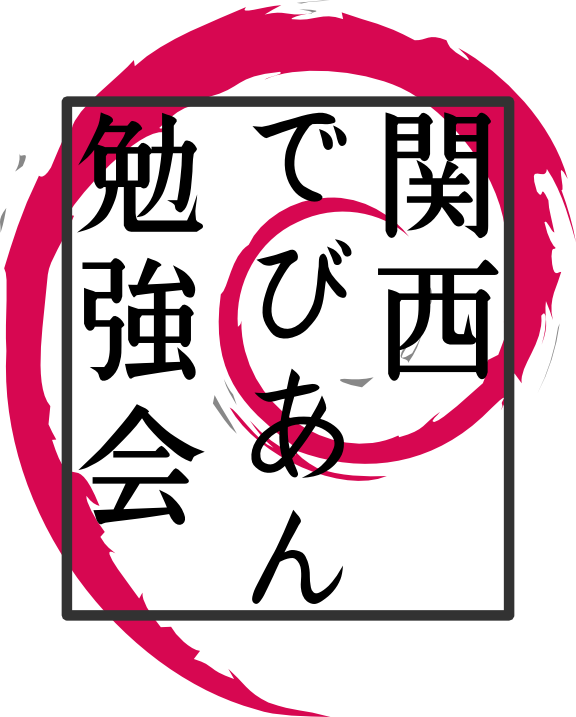
\includegraphics{image200802/kansaidebianlogo.png}
\end{center}

\begin{flushright}
\hfill{}$B4X@>(B Debian $BJY6/2qC4Ev<T(B $B:4!9LZ!&ARI_!&$N$,$?!&$+$o$@!&H,DEHx(B \\
\hfill{}\debmtgyear{}$BG/(B\debmtgmonth{}$B7n(B\debmtgdate{}$BF|(B
\end{flushright}

\thispagestyle{empty}
\end{titlepage}

\dancersection{Introduction}{Debian JP}

\vspace{1em}

 $B4X@>(BDebian$BJY6/2q$O(BDebian GNU/Linux$B$N$5$^$6$^$J%H%T%C%/(B
 ($B?7$7$$%Q%C%1!<%8!"(BDebian$BFCM-$N5!G=$N;EAH!"(BDebian$B3&7($G5/$3$C$?=PMh;v!"(B
 $B$J$I$J$I!K$K$D$$$FOC$79g$&2q$G$9!#(B

 $BL\E*$H$7$F<!$N;0$D$r9M$($F$$$^$9!#(B
 \begin{itemize}
  \item ML$B$d7G<(HD$G$O$J$/!"D>@\4i$r9g$o$;$k;v$G$N>pJs8r49$NB%?J(B
  \item $BDj4|E*$K=8$^$l$k>l=j(B
  \item $B;qNA$N:n@.(B
 \end{itemize}

 $B$=$l$G$O!"3Z$7$$0l;~$r$*2a$4$7$/$@$5$$!#(B

\newpage

\begin{minipage}[b]{0.2\hsize}
 {\rotatebox{90}{\fontsize{80}{80}
{\gt $B4X@>(B Debian $BJY6/2q(B}}}
\end{minipage}
\begin{minipage}[b]{0.8\hsize}
\hrule
\vspace{2mm}
\hrule
\setcounter{tocdepth}{1}
\tableofcontents
\vspace{2mm}
\hrule
\end{minipage}

\dancersection{$B:G6a$N(BDebian$B4X78$N%$%Y%s%HJs9p(B}{Debian JP}

\subsection{$BBh(B84$B2s4X@>(BDebian$BJY6/2q(B}

84$B2sL\$N4X@>(BDebian$BJY6/2q$O(B5$B7n(B25$BF|(B($BF|(B)$B$K!"J!Eg6hL1%;%s%?!<$G9T$J$o$l$^$7(B
$B$?!#(B

$B$b$/$b$/$N2qCf?4$N3+:E$G$7$?$,!"%-!<%5%$%s!"(Bsystemd$B$NOC$7$,OCBj$K$"$,$j(B
$B$^$7$?!#:#2s$O$=$NB3$-$H$$$&46$8$G(Bsystemd$B$N$*OC$7$K$J$j$^$9!#(B

\subsection{$BBh(B114$B2sEl5~%(%j%"(BDebian$BJY6/2q(B}

114$B2sL\$NEl5~%(%j%"(BDebian$BJY6/2q$O(B6$B7n(B14$BF|(B($BEZ(B)$B$K3t<02q<R%9%/%&%'%"!&%(%K%C(B
$B%/%9(B $B2q5D<<$G9T$J$o$l$^$7$?!#(B

$B5HED$5$s$K$h$k!V(BGPG $BHkL)80<h$j07$$J}K!$NDs0F!W$H$b$/$b$/$N2q$N7A<0$G9T(B
$B$J$o$l$^$7$?!#(B

$B$_$J$5$sG:$_$I$3$m$N(BGPG$BHkL)80$N07$$$r$I$&$9$k$+$K$D$$$F!"$3$N%;%C%7%g(B
$B%s$G$O(BGPG$BHkL)80$r(BRAID5$B$N$h$&$KJ#?t$N%U%!%$%k$H%Q%j%F%#$KJ,3d$7$F4IM}$9(B
$B$k%"%$%G%"$,>R2p$5$l$F$$$^$9!#LLGr$$J}K!$@$H;W$$$^$9$N$G$<$R;qNA$KL\$r(B
$BDL$7$F$_$F$/$@$5$$!#(B

\subsection{Debian Project}

\subsubsection{MATE 1.8}
MATE Packaging Team$B$h$j!V(BMATE 1.8 has now fully arrived in Debian$B!W(B
\footnote{\url{https://lists.debian.org/debian-devel/2014/06/msg00041.html}}
$B$H(BMATE 1.8$B$,(BDebian$B$KDI2C$5$l$?$h$H%"%J%&%s%9$,$"$j$^$7$?!#(B
MATE$B$O(BGNOME2$B$+$i%U%)!<%/$7$?%G%9%/%H%C%W4D6-%W%m%8%'%/%H$G$9!#(BGNOME3$B$r(B
$B9%$^$7$$$H;W$C$F$$$J$$J}$K$H$C$F$O9%I>$G!"$h$[$I$&$l$7$+$C$?$N$+(B10$BJ,$b(B
$B7P$?$J$$$&$A$K(BNorbert Preining$B$5$s$+$i(B
\begin{quote}
  *big*big*big* thanks for all your work, it is very very much appreciated!
\end{quote}
$B$H46<U$N%a!<%k$,Ht$s$G$$$^$7$?!#(B

$B$9$G$K!"(Bunstable$B$@$1$G$J$/(Btesting$B!"(Bwheezy-backports$B$K$b%Q%C%1!<%8$,MQ0U(B
$B$5$l$F$$$^$9$N$G;n$7$F$_$?$$J}$O<!$N%a%?%Q%C%1!<%8$r%$%s%9%H!<%k$7$F$_(B
$B$F$/$@$5$$!#(B
\begin{commandline}
  $ sudo apt-get install mate-desktop-environment
\end{commandline}
%$

\subsubsection{Debian 6 ``squeeze'' LTS}
Debian Project$B$+$i!V(BDebian 6 debuts its long term support period$B!W(B
\footnote{\url{https://lists.debian.org/debian-announce/2014/msg00004.html}}
$B$H(BDebian$B=i$H$J$k(BLTS (Long Term Support)$B$r(BDebian GNU/Linux 6.0 ``squeeze''
$B$KDs6!$7$^$9$H%"%J%&%s%9$,$"$j$^$7$?!#$3$N%5%]!<%H$O(B2016$BG/(B2$B7n$^$GB3$1(B
$B$i$l$kM=Dj$G$9!#(B

LTS$B$rMxMQ$7$F$_$h$&$H;W$o$l$kJ}$O!V(BHow to use the updates from LTS$B!W(B
\footnote{\url{lhttps://wiki.debian.org/LTS/Using}}
$B$K$h$/L\$rDL$7$F$+$iMxMQ$7$F$/$@$5$$!#A4%"!<%-%F%/%A%c!"A4%Q%C%1!<%8$,(B
LTS$B%5%]!<%H$NBP>]$G$O$"$j$^$;$s$N$G==J,$KCm0U$7$F$/$@$5$$!#(B
$B$I$N%Q%C%1!<%8$,(BLTS$B$N%5%]!<%H$NBP>]30$H$J$k$+$O(Bdebian-security-support
$B%Q%C%1!<%8$r;H$C$F3NG'$9$k$3$H$,$G$-$^$9!#(B

\subsubsection{Berkeley DB}
$B!V(BNew project goal: Get rid of Berkeley DB (post jessie)$B!W(B
\footnote{\url{https://lists.debian.org/debian-devel/2014/06/msg00328.html}}
$B$G(BBerkeley DB$B$O;`$s$@$N$G(BLMDB$B$N$h$&$JJL$N<BAu$KCV$-49$($h$&$H$$$&Ds0F(B
$B$,$"$j$^$7$?!#(B
$B$A$g$&$I0lG/$[$IA0$K!V(BBerkeley DB 6.0 license change to AGPLv3$B!W(B
\footnote{\url{https://lists.debian.org/debian-devel/2013/07/msg00031.html}}
$B$GOCBj$K$J$C$?(BAGPLv3$B$X$N%i%$%;%s%9JQ99$K$h$k$b$N$G$9!#$3$N$?$aL$$@(B
Berkeley DB 6.0$B$O(BDebian$B$N%j%]%8%H%j$KF~$C$F$$$^$;$s!#(B
\footnote{$B%P!<%8%g%s(B6.0.19$B$,(Bexperimental$B$KF~$C$?$3$H$,$"$k$N$G$9$,!"$=(B
$B$N8e(B5.3.21$B$KLa$5$l$^$7$?!#(B}

$B@h7n$b(BGhostscript$B$,(BAGPL$B$K%j%i%$%;%s%9$5$l$?OCBj$,$"$j$^$7$?$,!"%i%$%;(B
$B%s%9JQ99$NLdBj$OG:$^$7$$$G$9!#(B

\dancersection{$B;vA02]Bj(B}{Debian JP}

$B:#2s$N2]Bj$O0J2<$NDL$j$G$9!#(B
\begin{screen}
  \begin{enumerate}

  \item %
    $B$b$/$b$/$N2q$G9T$J$&:n6H!"<ALd$J$I$N2]Bj$rMQ0U$7$F65$($F$/$@$5$$!#(B
    ($BEE8;$H%M%C%H%o!<%/(B(WiMAX$B$J$I(B)$B$O$"$j$^$9$,!"$=$l0J30$N:n6H$KI,MW$J(B
    $B4D6-$O$4MQ0U$/$@$5$$!#(B)

  \item %
    $BA02s(B($BBh(B84$B2s(B)$B$NJY6/2q$K;22C$5$l$?J}$O!"A02s$N:n6H$d2]Bj$,$=$N8e$I$&(B
    $B$J$C$?$+7k2L$r65$($F$/$@$5$$!#(B

  \item %
    LT($B%i%$%H%K%s%0%H!<%/(B) $B4?7^$G$9!#2?$+$*OC$7$?$$J}$O%?%$%H%k$r2<$5$$!#(B

  \item %
    Debian$B$G(BInit$B$H$7$F(Bsystemd$B$,F0:n$9$k4D6-$rMQ0U$7$F$-$F2<$5$$!#(B
    $B2>A[4D6-$G$+$^$$$^$;$s!#(Bunstable$B$r$*;H$$$NJ}$O(Bsystemd-sysv$B%Q%C%1!<(B
    $B%8$rF3F~$9$k$H(Bsysvinit-core$B$,(Breplace$B$5$l$F(BInit$B$H$7$F(Bsystemd$B$,F0:n(B
    $B$9$k$h$&$K$J$j$^$9!#(B

  \end{enumerate}
\end{screen}

$B;22C<T$N3'$5$s$N2rEz$O0J2<$NDL$j$G$9(B:

\begin{prework}{ $B$+$o$@$F$D$?$m$&(B }
  \begin{enumerate}
  \item uim-skk$B$r;HMQ$7$F$$$k$N$G$9$,!"(B
    \begin{itemize}
    \item chromium$B$G(Btitanpad$B$K$+$JF~NO$G$-$J$$(B
    \item xmonad+gnucache$B$G$+$JF~NO$G$-$J$$(B
    \end{itemize}
    $B$N$r$J$s$H$+$7$?$$(B
  \end{enumerate}
\end{prework}

\begin{prework}{ $B:4!9LZMNJ?(B }
  $B?=$79~$_$o$9$l$F$?$o!<!#(B

  \begin{enumerate}
  \item jekyll $B$N0MB8$,(B newqueue $B$+$i(B unstable $B$KMn$A$?$N$G!"$h$&$d$/(B
    new upstream $B$r(B upload $B$G$-$^$9!#(B
  \end{enumerate}

\end{prework}

\begin{prework}{ $BLZ2<(B }
  \begin{enumerate}
  \item
    \begin{enumerate}
    \item Eucalyptus$B!J%W%i%$%Y!<%H%/%i%&%I$H$7$F!K$ND4::!&8&5f(B
    \item $B%0%j%C%I%3%s%T%e!<%F%#%s%04XO"$ND4::!&8&5f(B
      \begin{itemize}
      \item GlobusToolkit$B$G2?$,$G$-$k!)(B

        $B"*(BAndroidOS$B$N%/%m%9%3%s%Q%$%k$G;H$($?$i4r$7$$$+$b!#(B
      \end{itemize}
    \item Debian7 on PANDABOARD$B$ND4::!&8&5f(B
      \begin{itemize}
      \item WiFi$B%b%8%e!<%k!J(BOn Board$B!'(BTI$B@=!K$NM-8z2=(B
      \item GPU$B%G%P%$%9%I%i%$%P$NM-8z2=(B
      \end{itemize}
    \end{enumerate}
  \item $B"(A02s(B($BBh(B84$B2s(B)$B$O7g@J$@$C$?0Y!"Bh(B83$B2s$NFbMF$K$J$j$^$9!#(B
    \begin{enumerate}
    \item Eucalyptus$B!J%W%i%$%Y!<%H%/%i%&%I$H$7$F!K$ND4::!&8&5f(B

      $B<B@S!'%$%s%9%?%s%9$NJ]B8$H<+F02=$K@.8y(B
      \begin{itemize}
      \item $BJ]B8$7$?%$%s%9%?%s%9$r5/F0$5$;$k$H%M%C%H%o!<%/@\B3$,@d$?$l$F$7$^$C$F$$$?860x(B

        $B"*%U%!%$%k!'(B/etc/udev/rules.d/70-persistent-net.rules$B$K(BNIC$B%G%P%$%9>pJs$,;D$C$F$$$k$H(B
        $B?7$?$K(BNIC$B%G%P%$%9>pJs$,EPO?$5$l$F$7$^$$!"(BNIC$BHV9f$,JQ99$5$l!"DL?.IT2D$H$J$C$F$$$?!#(B

        $B"((BEucalyptus$B4X78<T$NJ}$N$*OC$G$O!"!V(BDebian$BMQ%D!<%k$N%P%0$+$b!W$H$N$3$H!#(B
        $B%$%s%9%?%s%9J]B8$K%/%j%"$9$k$3$H$G2r7h$7$?!#(B
      \item $B%$%s%9%?%s%9$r(BOS$B%$%a!<%8%U%!%$%k2=$7!"%O%$%Q!<%P%$%6>e$K%P%C%/%"%C%W$9$k(B

        $B%9%/%j%W%H$r:n@.$7!"(Bcrontab$B$GDj4|E*$K5/F0$G$-$k$h$&$K$J$C$?!#(B
      \end{itemize}
    \item DistCC$B$ND4::!&8&5f(B

      $B<B@S!'>e5-%W%i%$%Y!<%H%/%i%&%I%7%9%F%`$rMQ$$$FJ#?t$N(BVM$B$GJ,;6%3%s%Q%$%k$5$;$k(B
      $B4D6-9=C[$K@.8y!#(B
      \begin{itemize}
      \item $B%S%k%I%^%7%s!J(Bdistcc$B%/%i%$%"%s%H!K$H(BVM$B!J(Bdistcc$B%5!<%P!K(B4$BBf$G(B
        PANDABOARD$B!J(BOS$B!'(BAndroid4.0.4$B!KMQ(BFW$B$rJ,;6%3%s%Q%$%k$5$;!"(B
        $B%3%s%Q%$%k;~4V$NC;=L$,2DG=$H$J$C$?!#(B
      \end{itemize}
      $B2]Bj!'(BAndroidOS$B$N>l9g!"(BJAVA$B$N%3%s%Q%$%k2U=j$,$+$J$jB8:_$9$k$N$G!"(B
      $B$3$NItJ,$,J#?t%^%7%s$GJ,;6%3%s%Q%$%k$G$-$k$h$&$K$J$l$P!"(B
      $B$+$J$j$N%3%s%Q%$%k;~4V$NC;=L$H$J$j$=$&$J$N$G!"$3$N$"$?$j$K$D$$$F:FD4::I,MW!#(B
    \item $B%0%j%C%I%3%s%T%e!<%F%#%s%04XO"$ND4::!&8&5f(B

      $B<B@S!'J]N1(B
    \item Debian7 on PANDABOARD$B$ND4::!&8&5f(B

      $B<B@S!'J]N1(B
    \end{enumerate}
  \end{enumerate}
\end{prework}

\begin{prework}{ takata }
  \begin{enumerate}
  \item $B2]Bj!'(BLUKS$B%Q!<%F%#%7%g%s$N%Q%9%o!<%IF~NO$r>JN,$9$k7o!JL$2r7h!K(B

    keyfile$B$rEPO?$7$F$_$^$7$?$,!"0MA3$H$7$F(B swap$B%Q!<%F%#%7%g%s$K4X$7$F(B
    $B$O5/F0;~$K%Q%9%o!<%I$rJ9$+$l$^$9!#%0%0$C$F$_$k$HF1MM$NLdBj$,$$$/$D(B
    $B$+%R%C%H$9$k$h$&$J$N$G!"$b$/$b$/$N2q$N;~4V$G$b$&>/$7D4$Y$F$_$?$$$H(B
    $B;W$C$F$$$^$9!#(B

    stop crypttab asking for password for swap

    \url{http://askubuntu.com/questions/43432/stop-crypttab-asking-for-password-for-swap}

    $B$A$J$_$K!"(B"/"$B%Q!<%F%#%7%g%s$N(B keyfile$B$G%H%i%V$j$^$7$?!#(B
    $B4V0c$($FDI2C$7$9$.$F$7$^$C$?(B key\_{}slot$B$r(B cryptsetup luksRemoveKey
    $B$G:o=|$7$h$&$H$7$?$N$G$9$,!"%Q%9%o!<%I$rEPO?$7$?(B key\_{}slot$B$r8m$C(B
    $B$F:o=|$7$F$7$^$$!"(Bcryptsetup luksAddKey$B$G%-!<$rEPO?$G$-$J$/$J$k$P$+(B
    $B$j$+%Q%9%o!<%I$,2r=|$G$-$J$/$J$C$F$7$^$$!J(BNo key available with this passphrase.$B!K!"(B
    $B0l=VNd$d4@$,=P$^$7$?!#9,$$!"(Bkeyfile$B$r@_Dj$7$?(B Key Slot$B$,;D$C$F$$$?$N$G!"(B
    cryptsetup luksAddKey --key-file=...$B$G2sHr$G$-2?$H$+;v$J$-$rF@$^$7$?$,!"(B
    Key Slot$B$r:o=|$9$k>l9g$O$/$l$0$l$b$4Cm0U$/$@$5$$!#(B

  \item $B%$%s%?!<%M%C%H$+$i$N(B22$BHV%]!<%H(B(ssh)$B$X$NIT@5%"%/%;%9$K$D$$$F(B

    $B65$($F$$$?$@$$$?$H$*$j!"(Bfail2ban$B$rE,MQ$9$k$3$H$GIT@5%"%/%;%9$KBP$7(B
    $B$FM-8z$K%V%m%C%/$G$-$F$$$k$h$&$G$9!#$"$j$,$H$&$4$6$$$^$7$?!#(B
  \end{enumerate}
\end{prework}

\clearpage

\begin{prework}{ $B@>;3OB9-(B }
  \begin{enumerate}
  \item ansible $B$G$N%5!<%P!<@_Dj$r?J$a$?$$$G$9!#(B
  \item $BA02sIT;22C$G$9!#(B
  \item blog $B$N5-;v$+$i(B \verb+^+Xg $B$NOC$rM=Dj$7$F$$$^$9!#(B
  \item $BMQ0U$7$F$*$-$^$9!#(B
  \end{enumerate}
\end{prework}

\begin{prework}{ yyatsuo }
  \begin{enumerate}
  \item kernel-handbook $B$NF|K\8lLu$r$=$m$=$m$J$s$H$+$7$^$9(B
    $B$"$H$OK?;(;o$N5-;v::FI$H$+(B
  \item fcitx-skk new que $B$KF~$j$^$7$?!*(B
    (new que $B$G;_$^$C$F$k$H$b8@$$$^$9(B)
  \item $B;E;v$N6rCT$J$iN/$^$C$F$^$9$h!)(B
  \item $B$b$&F~$C$F$k(B
  \end{enumerate}
\end{prework}

\begin{prework}{ $B1]??<#(B }

  Debian wheezy$B$G(BAnthy$B$r;H$C$F$$$^$9$,!"F|K\8lF~NO$NJQ498zN(!J8uJd$,4|(B
  $BBT$7$?$h$&$J=gHV$GJB$s$G$/$l$J$$$J$I!K$,$$$^$R$H$D$H46$8$F$$$^$9$N$G!"(B
  $B4D6-$rJQ99$7$F$_$?$$$H9M$($F$$$^$9!#(B

  $B$*4+$a$NJ}K!$O$"$j$^$9$+!)(B

  mozc$B$r;n$9$H$7$?$i(Buim,ibus$B$J$I$N$I$l$,$*4+$a$G$9$+!)(B
\end{prework}

\begin{prework}{ $B:dK\(B $B5.;K(B }
  \begin{enumerate}
  \item $B1Q8l%I%-%e%a%s%H$r(BTex$B%U%)!<%^%C%H$G:n@.$7$F$$$k$N$G!"$=$NB3$-$r=q$-$^$9!#(B
  \item $BA02s$O;22C$7$F$$$^$;$s(B
  \item $B!V(BLinux$B$N%I%i%$%P%a%s%F%J$K$J$C$?BN835-!W$H$$$&%?%$%H%k$GC;$$%;%C%7%g%s$r$9$kM=Dj$G$9(B
  \end{enumerate}
\end{prework}

\begin{prework}{ lurdan }
  \begin{enumerate}
  \item $B<j;}$A%Q%C%1!<%8$N(B bug squash
  \item webwml-git $B$O(B CI $B$G$-$k$h$&$K$O$J$C$?$1$I!"1?MQ$,HQ;($J$N$G:F8!F$Cf$G$9(B
  \end{enumerate}
\end{prework}

\begin{prework}{ $B@n9>(B }
  \begin{enumerate}
  \item emacs$B$K$F!"(BHTML5$B7A<0$N%5%$%H$N:n@.!#$G!"(Bwed-mode.el$B$,(Bdebian$B$N(B
    $B%Q%C%1!<%8$K$J$$$N$G$9$,!"$3$l$C$F!V(Banthy-el$B!W$N$h$&$K%Q%C%1!<%8$K(B
    $B$G$-$^$9!)!!$H$$$&$+!V(B.el$B!W%U%!%$%k$H$$$&$N$O$=$b$=$b2?!)(B
  \end{enumerate}
\end{prework}

\begin{prework}{ Hiroyuki Nagata }
  \begin{enumerate}
  \item RFS$B$N$d$jJ}!"(BGPG$B80$N8r49!!!D!!:#EY$O$"$kDxEY=`Hw$r$7$F$/$k$D$b$j(B
  \item GPG$B80$r:n@.$7$^$7$?!"(BMac Book Pro$B$K(BDebian jessie$B$r%$%s%9%H!<%k$7$^$7$?(B
  \item $B:#7n$O$`$j$+$b$7$l$^$;$s$,(BDebian$B$G%k!<%?9=C[$H$+(B
  \end{enumerate}
\end{prework}

\dancersection{Debian $B$G$N(B systemd $B$H$N$D$-$"$$J}(B}{$B:4!9LZ(B $BMNJ?(B}

\begin{quote}
  Yes, it is written systemd, not system D or System D, or even
  SystemD. And it isn't system d either. \\
  \begin{flushright}
    Spelling - \texttt{http://www.freedesktop.org/wiki/Software/systemd/}
  \end{flushright}
\end{quote}

\subsection{$B$O$8$a$K(B}

$B>/$7A0$NOC$G$9$,!"<!4|(BDebian$B0BDjHG(BJessie$B$G$N%G%U%)%k%H$N(BInit$B$H$7$F(Bsystemd$B$,:NMQ$5$l$^$7$?!#(B
$BJY6/2q;22C<T$N3'MM$K$*$+$l$^$7$F$O!"(B% $B!V:G6a(BDebian$B4XO"$N%$%Y%s%HJs9p!W$G>R2p(B(?)$B$5$l$?!"(B
\texttt{debian-devel@lists.debian.org}$B$XN.$l$?(B\sout{$BIJ$NL5$$(B}$BHaLD(B(?)$B$b5-21$K?7$7$$$3$H$G$7$g$&(B
\footnote{%
Fsck SystemD and its developers and its users. GR to override this please.\\
$B!!(B\href{https://lists.debian.org/debian-devel/2014/02/msg00316.html}{\texttt{https://lists.debian.org/debian-devel/2014/02/msg00316.html}}%
}$B!#(B

$B?'!9$J0U8+$O$"$k$G$7$g$&$1$l$I$b!"(B
$B!V%G%U%)%k%H!W$H$7$F:NMQ$5$l$k0J>e(B($B9%$`$H9%$^$6$k$H$K$+$+$o$i$:(B)Debian$B$N3+H/<T(B($B4^%o%J%S!<(B)$B$K$H$C$F(Bsystemd$B$NCN<1$OI,?\;v9`$K$J$j$=$&$G$9!#(B
$B$=$s$JLu$G!"(Bsystemd$B$=$N$b$N$K$D$$$FD4$Y$?7k2L$H(BDebian$B$K$*$1$k8=>u$K$D$$$F$^$H$a$F$_$^$9!#(B%
$B$A$J$_$K<g$K%F%9%H$7$?4D6-$O0J2<$NDL$j(B:
\begin{commandline}
% LANG=C date
Sat Jun 21 10:15:59 JST 2014
% lsb_release -a
No LSB modules are available.
Distributor ID: Debian
Description:    Debian GNU/Linux unstable (sid)
Release:        unstable
Codename:       sid
% dpkg -l | grep systemd
ii  libpam-systemd:amd64        204-10   amd64   system and service manager - PAM module
ii  libsystemd-daemon0:amd64    204-10   amd64   systemd utility library
ii  libsystemd-id128-0:amd64    204-10   amd64   systemd 128 bit ID utility library
ii  libsystemd-journal0:amd64   204-10   amd64   systemd journal utility library
ii  libsystemd-login0:amd64     204-10   amd64   systemd login utility library
ii  systemd                     204-10   amd64   system and service manager
ii  systemd-gui                 1:3-2    all     transitional package for systemd-ui
ii  systemd-sysv                204-10   amd64   system and service manager - SysV links
ii  systemd-ui                  3-2      amd64   graphical frontend for systemd
\end{commandline}
\noindent
$BK\869F$N<9I.;~4V$,$h$/$o$+$j$^$9(B\footnote{%
  lsb-base$B$H(Blsb-release$B$7$+%$%s%9%H!<%k$7$F$$$J$$$N$G(B%
  \texttt{lsb\_release -a}$B$N=PNO7k2L$O$3$s$J%b%s$G$9!#(B
}$B!#(B
%
$B0l1~(Bwhezzy + wheezy-backports$B$G$b%F%9%H$O$7$F$_$^$7$?$,!#(B

...$B$7$+$7(B, v204 $B$C$F(B...$B!#(B

\subsection{$B$=$b$=$b(B systemd $B$C$F%J%K$h(B?}

systemd$B$O(BLennart Poettering$B;a(B%
\footnote{Red Hat Inc.$B$N%(%s%8%K%"$5$s$G$9!#(B%
  systemd$B$N3+H/<T$@$1$G$J$/MM!9$J%U%j!<%=%U%H%&%'%"$N3+H/<T$G$b$"$j$^$9!#(B%
  $BNc$($P(BPulseAudio$B$H$+(BAvahi$B$J$s$+$N%a%$%s3+H/<T$G$b$"$j$^$9$M!#(B}%
$B$K$h$C$F3+H/$5$l$F$$$k(BInit$B$NBeBX%W%m%0%i%`$G(B\sout{$B$9(B}$B$7$?!#(B
$B:#$G$OC1$J$k!V(BInit$B$NBeBX!W$H$$$&$h$j!V(BLinux$B$N%5!<%S%9(B($B%G!<%b%s(B)$B4IM}%U%l!<%`%o!<%/!W$H$J$C$F$$$^$9!#(B
$B3+H/$O(B
\texttt{freedesktop.org}\footnote{%
  \href{http://www.freedesktop.org/wiki/Software/systemd/}{\texttt{http://www.freedesktop.org/wiki/Software/systemd/}}%
}$B$G9T$J$o$l$F$*$j!"%i%$%;%s%9$O(BLGPL-2.1+$B!":G?7%P!<%8%g%s$O(Bv214$B$H$J$C$F$$$^$9!#(B

$B!V(BLinux$B$N%5!<%S%9(B($B%G!<%b%s(B)$B4IM}%U%l!<%`%o!<%/!W$H$7$F$N(Bsystemd$B$NFCD'$O(B
\begin{enumerate}[topsep=1zw]
\item Init$B$H$7$F!"(BSysV$B$*$h$S(BLSB init script $B$H$N8_49@-$NDs6!!#(B
\item $B%5!<%S%9$N5/F0$r%=%1%C%H$H%P%9(B(D-Bus)$B$G9T$J$&!#(B
\item $B%5!<%S%94V$N0MB84X78$rL@3N$K$7!"$h$j%"%0%l%C%7%V$KJBNs5/F0$9$k!#(B
\item $B%*%s%G%^%s%I$J%5!<%S%9$N5/F0!#(B
\item $B%W%m%;%94IM}$r(Bpid$B$G$O$J$/(Bcgroups(control groups)$B$G9T$J$&!#(B
\end{enumerate}
$B$H$$$C$?=j$G$9!#(B

$B4{$K(BLinux$B%+!<%M%kMQ$N%G%P%$%94IM}%D!<%k$G$"$k(Budev$B$,(Bsystemd$B$N%=!<%9$K%^!<%8$5$l$F$*$j!"(B
$B%G%P%$%9$N>uBV$K1~$8$F%*%s%G%^%s%I$K%5!<%S%9$,5/F0$7$?$j$7$^$9!#(B
$B>-MhE*$K$O(Bcron$B$d(Bacpid$B$NBeBX5!G=$bDs6!$9$kM=Dj$i$7$$$G$9(B\footnote{%
  $B$3$3$^$GMh$k$H$d$j$9$.$J46$bH]$a$^$;$s$,(B...$B!#(B
}$B!#(B
$B$=$NB>!"(Bsystemd$B$K4X$9$k3+H/<T$N;WA[!"8=>u$K4X$7$F$O(B
\begin{itemize}
\item %
  \href{http://0pointer.de/blog/projects/systemd.html}{\texttt{http://0pointer.de/blog/projects/systemd.html}}
\item %
  \href{http://0pointer.de/blog/projects/systemd-for-admins-1.html}{\texttt{http://0pointer.de/blog/projects/systemd-for-admins-1.html}}
  $B$+$i;O$^$k0lO"$N%(%s%H%j(B\footnote{$B8=:_(B\#20$B$^$G$"$j$^$9!#D9$/$FFI$`$N?I$$(B...$B!#(B}
\end{itemize}
$B$,Hs>o$K;29M$K$J$k$G$7$g$&!#(B

\subsection{Debian $B$G;H$&$K$O(B?}

systemd$B$NI,MWMW7o$O0J2<$NDL$j$G$9(B:
\begin{enumerate}[topsep=1zw]
\item Linux$B%+!<%M%k$N%P!<%8%g%s$O(B2.6.39$B0J>e(B
\item $B0J2<$N5!G=$,M-8z$H$J$C$F$$$k$3$H(B
  \begin{itemize}[topsep=0zw]
  \item devtmpfs
  \item fanotify
  \item autofs4
  \item cgroups
  \end{itemize}
\end{enumerate}
$B%+%9%?%`%+!<%M%k$r;HMQ$5$l$F$$$k>l9g$K$O!"%+!<%M%k$N%P!<%8%g%sEy$K$4Cm0U2<$5$$!#(B

Debian$B$G%Q%C%1!<%8$H$7$FDs6!$5$l$F$$$k(Bsystemd$B$N%P!<%8%g%s$O(B
\begin{itemize}[topsep=1zw]
\item wheezy: v44
\item wheezy-backports: 204-8\~{}bpo70+1
\item jessie/sid: 204-10
\end{itemize}
$B$G$9!#0J2<!"%Q%C%1!<%8$H$7$FDs6!$5$l$F$$$k:G?7HG$G$"$k(Bv204$B$N$*OC$r$7$^$9(B\footnote{%
  $B$A$J$_$K!"(Bv44$B$r;HMQ$9$k>l9g$N<j=g$O!"(B
  \texttt{systemd} $B$r(B install $B"*(B
  $B5/F0;~$K(B \texttt{init=/lib/systemd/systemd}$B$H;XDj$9$k(B or grub $B%(%s%H%j$N=q$-49$($r9T$J$&!"$G$9!#(B
}
$B$G$OF3F~$7$F$_$^$7$g$&!#(Bwheezy$B$r$*;H$$$NJ}$O(Bwheezy-backports$B$rM-8z$K$7$F2<$5$$!#(B
init$B$r(Bsysvinit$B$+$iCV$-49$($k$?$a$K!"(B\texttt{systemd-sysv}$B$rF3F~$7$^$9!#(B
\begin{commandline}
% sudo aptitude install systemd-sysv -t wheezy-backports <-- wheezy $B$N>l9g(B
% sudp aptitude install systemd-sysv                     <-- jessie/sid $B$N>l9g(B
\end{commandline}
wheezy$B$N>l9g$K$O(Bsysvinit$B$,(Bcore$B%Q%C%1!<%8$J$N$G!"%$%s%9%H!<%k;~$N0MB84X782r7h$KB?>/<j4V$I$k$+$b$7$l$^$;$s!#(B
$B0J2<$N%Q%C%1!<%8$,0MB84X78$G%$%s%9%H!<%k$5$l$^$9!#(B
\begin{commandline}
===============================================================================
[$B%$%s%9%H!<%k(B] libpam-systemd:amd64
[$B%$%s%9%H!<%k(B] libsystemd-journal0:amd64
[$B%$%s%9%H!<%k(B] libudev1:amd64
[$B%$%s%9%H!<%k(B] systemd:amd64
[$B%$%s%9%H!<%k(B] systemd-sysv:amd64
[$B:o=|(B] sysvinit:amd64
[$B99?7(B] libsystemd-daemon0:amd64 44-11+deb7u4 -> 204-8~bpo70+1
[$B99?7(B] libsystemd-login0:amd64 44-11+deb7u4 -> 204-8~bpo70+1
===============================================================================
\end{commandline}
$B%$%s%9%H!<%k$,=*$o$C$?$i(B reboot $B$7$^$9!#(B...$BL5;v5/F0$G$-$?$G$7$g$&$+(B?

systemd$B$O(Bboot$B%W%m%;%9$N2r@O%D!<%k$,$"$j!"5/F0;~$K$+$+$C$?;~4V$,D>$0$K$o$+$j$^$9!#(B
\begin{commandline}
% systemd-analyze
Startup finished in 1.632s (kernel) + 3min 2.710s (userspace) = 3min 4.343s
\end{commandline}
...$B$"$l(B?
\begin{commandline}
% systemd-analyze blame
       3min 12ms dnsmasq.service
        2.074s systemd-udev-settle.service
         630ms psd.service
         307ms NetworkManager.service
         127ms squid3.service
         106ms bluetooth.service
          98ms udisks2.service
          96ms exim4.service
          93ms keyboard-setup.service
          87ms bootlogs.service
          87ms avahi-daemon.service
          80ms resolvconf.service
          76ms console-setup.service
          74ms networking.service
          73ms systemd-logind.service
          69ms netfilter-persistent.service
          64ms console-kit-log-system-start.service
          ...$B0J2<N,(B...
\end{commandline}
$B;8A3$H51$/(B\textbf{3min 12ms dnsmasq.service}$B!#!D$*$+$7$$!#$3$l$O$*$+$7$$!#(B

\subsection{$B8=>u$I$&$J$N$h(B?}

$B5$$r<h$j$J$*$7$F!#(B

\subsubsection{systemd$B$NMQ8l(B}
systemd$B$rM}2r$9$k$?$a$K!"@h$:$OMQ8l$r3NG'$7$^$7$g$&!#(B
\begin{itemize}
\item $B%f%K%C%H(B(unit): \\
  SysVinit$B$N=i4|2=%9%/%j%W%H$K$^$H$a$F4^$^$l$F$$$?8D!9$N=hM}$rH4$-=P$7$?:G>.C10L!#(B
  $B8D!9$N(BUnit$B$O$=$l$>$l0J2<$NDL$j(B:
  \begin{itemize}
  \item $B%5!<%S%9(B(\texttt{.service}): \\
    $B%G!<%b%s$r5/F0$9$k(B
  \item $B%=%1%C%H(B(\texttt{.socket}): \\
    systemd$B$,;XDj$5$l$?(Bsocket$B$r4F;k$7!"@\B3$,$"$k$H;XDj$N(B\texttt{.service}$B$r5/F0$7!"(Bsocket$B$rEO$9!#(Binetd$B$NMM$JLr3d!#(B
  \item $B%?!<%2%C%H(B(\texttt{.target}):\\
    $BJ#?t$N%f%K%C%H$r$^$H$a$F!"0MB84X78$d=g=x4X78$rDj5A$9$k!#(BSysVinit$B$N(Brunlevel$B$KBP1~(B\footnote{%
      $B87L)$K(B1$BBP(B1$B$KBP1~$9$kLu$G$O$J$$!#(B%
    }
  \item $B%^%&%s%H%]%$%s%H(B(\texttt{.mount}): \\
    $B%U%!%$%k$r%^%&%s%H$9$k(B
  \item $B%9%o%C%W(B(\texttt{.swap}): \\
    $B%9%o%C%W$rM-8z2=(B
  \item $B%G%P%$%9(B(\texttt{.device}): \\
    udev$B$,%G%P%$%9$rG'<1$9$k$HM-8z2=$5$l$k!#(B
  \end{itemize}
\end{itemize}
$B$3$N$&$A!"(B\texttt{.mount},\texttt{.swap}$B$O(B\texttt{/etc/fstab}$B$+$i!"(B\texttt{.device}$B$O(Budev$B$+$i!"$=$l$>$l<+F0@8@.$5$l$^$9!#(B
$B$3$l$i!V%f%K%C%H!W$rDj5A$7$?%U%!%$%k$O(B\texttt{/lib/systemd}$B0J2<$KCV$+$l!"(B\texttt{/etc/systemd}$B0J2<$NE,@Z$J>l=j$X(Bsymbolic link$B$r$O$k$3$H$GM-8z$K$J$j$^$9!#(B

$B$^$?!"%?!<%2%C%H$O(BSysvInit$B$N(Brunlevel$B$K(B($B$J$s$H$J$/(B)$BBP1~$7$F$*$j!"(BDebian$B$N>l9g$K$O(B
\begin{table}[h]
  \centering
  \begin{tabular}{l|l}
    SysVinit $B$N(B runlevel & systemd $B$N(B target \\
    \hline
    0                    & poweroff.target \\
    1                    & rescue.target \\
    2 - 5                & multi-user.target \\
    6                    & reboot.target \\
    \hline
  \end{tabular}
  \caption{Debian$B$G$N(Brunlevel$B$H(B.target$B$NBP1~(B}
\end{table}
$B$H$J$C$F$$$^$9!#5/F0;~$K2?$b;XDj$7$J$$>l9g$K$O(Bdefault.target$B$,<B9T$5$l$^$9!#(B
$B<j85$N4D6-$G$O(Bdefault.target $B$O(B graphical.target$B$X$N(Bsymbolic link$B$K$J$C$F$$$^$7$?(B.
\begin{commandline}
  % ls -la /lib/systemd/system/default.target
  lrwxrwxrwx 1 root root 16 2014-04-27 19:43 /lib/systemd/system/default.target -> graphical.target
\end{commandline}
$B$G$O(B graphical.target $B$NCf?H$r8+$F$_$^$7$g$&(B
\begin{commandline}
% cat /lib/systemd/system/graphical.target | grep -v ^#

[Unit]
Description=Graphical Interface
Documentation=man:systemd.special(7)
Requires=multi-user.target
After=multi-user.target
Conflicts=rescue.target
Wants=display-manager.service
AllowIsolate=yes

[Install]
Alias=default.target

\end{commandline}
$B!V(BRequires$B!W!"!V(BAfter$B!W!"!V(BConflicts$B!W!"!V(BWants$B!W$,0MB8(B/$B=g=x4X78$rI=8=$7$F$$$^$9!#(B
$B$=$l$>$l(B
\begin{itemize}
\item Require: $B$3$3$G;XDj$5$l$F$$$k%f%K%C%H$,5/F0$7$F$$$k$3$H$,I,MW(B($B0MB84X78(B)$B!#(B
  Require$B$G;XDj$5$l$?%f%K%C%H$N5/F0$K<:GT$9$k$H!"$3$N%f%K%C%H$O<B9T$5$l$J$$!#(B
\item Wants: $B$3$3$G;XDj$5$l$F$$$k%f%K%C%H$,5/F0$7$F$$$k$3$H$,5a$a$i$l$k(B($B0MB84X78(B)$B!#(B
  $B$?$@$7!"(B
  Wants$B$G;XDj$5$l$?%f%K%C%H$N5/F0$K<:GT$7$F$b!"$3$N%f%K%C%H$O<B9T3+;O$5$l$k!#(B
\item After: $B$3$3$G;XDj$5$l$?%f%K%C%H$N5/F0!V8e!W$K<B9T$5$l$k(B($B=g=x4X78(B)$B!#(B
\item Before: $B$3$3$G;XDj$5$l$?%f%K%C%H$N5/F0!VA0!W$K<B9T$5$l$k(B($B=g=x4X78(B)$B!#(B
\end{itemize}
$B$H$J$C$F$$$^$9!#(B

$B%f%K%C%H$NA`:n$OA4$F(B\texttt{systemctl}$B%3%^%s%I$G9T$J$$$^$9!#(B
$B$G$O!"8=>u$N0MB8(B/$B=g=x4X78$rI=<($7$F$_$^$7$g$&!#(B
\begin{commandline}
  % systemctl list-dependencies [unit$BL>(B]
    unit$BL>>JN,;~$O(B default.target
  % systemctl list-dependencies [unit$BL>(B] --after
  % systemctl list-dependencies [unit$BL>(B] --before
\end{commandline}
\begin{commandline}
% systemctl list-dependencies
default.target
$B('(!(Bbootlogs.service
$B('(!(Bchrony.service
$B('(!(Bdovecot.service
$B('(!(Bexim4.service
$B('(!(Bhyperestraier.service
$B('(!(Blightdm.service
$B('(!(Bmotd.service
$B('(!(Bpsd.service
$B('(!(Bpulseaudio.service
$B('(!(Bschroot.service
$B('(!(Bsystemd-update-utmp-runlevel.service
$B('(!(Byaskkserv.service
$B(&(!(Bmulti-user.target
  $B('(!(Banacron.service
  $B('(!(Batd.service
   ...
\end{commandline}
$B8D!9$N(B unit $B$N>u67$O(B status $B$GI=<($G$-$^$9(B:
\begin{commandline}
% systemctl status ssh
ssh.service - OpenBSD Secure Shell server
   Loaded: loaded (/lib/systemd/system/ssh.service; enabled)
   Active: active (running) since $BF|(B 2014-06-22 14:17:07 JST; 25s ago
 Main PID: 9180 (sshd)
   CGroup: name=systemd:/system/ssh.service
           $B(&(!(B9180 /usr/sbin/sshd -D

 6$B7n(B 22 14:17:07 daphne systemd[1]: Started OpenBSD Secure Shell server.
 6$B7n(B 22 14:17:07 daphne sshd[9180]: Server listening on 0.0.0.0 port 22.
\end{commandline}

$B8D!9$N(B unit $B$N3+;O(B/$BDd;_(B/$B:F5/F0$O$=$l$>$l(B
start/stop/restart $B$G2DG=$G$9(B.
\begin{commandline}
% sudo systemctl stop ssh
% systemctl status ssh
ssh.service - OpenBSD Secure Shell server
   Loaded: loaded (/lib/systemd/system/ssh.service; enabled)
   Active: inactive (dead) since $BF|(B 2014-06-22 14:18:27 JST; 40s ago
  Process: 9180 ExecStart=/usr/sbin/sshd -D $SSHD_OPTS (code=exited, status=0/SUCCESS)

 6$B7n(B 22 14:17:07 daphne systemd[1]: Started OpenBSD Secure Shell server.
 6$B7n(B 22 14:17:07 daphne sshd[9180]: Server listening on 0.0.0.0 port 22.
 6$B7n(B 22 14:18:27 daphne systemd[1]: Stopping OpenBSD Secure Shell server...
 6$B7n(B 22 14:18:27 daphne systemd[1]: Stopped OpenBSD Secure Shell server.
% sudo systemctl start ssh
% systemctl status ssh
ssh.service - OpenBSD Secure Shell server
   Loaded: loaded (/lib/systemd/system/ssh.service; enabled)
   Active: active (running) since $BF|(B 2014-06-22 14:19:52 JST; 13s ago
 Main PID: 10819 (sshd)
   CGroup: name=systemd:/system/ssh.service
           $B(&(!(B10819 /usr/sbin/sshd -D
\end{commandline}
%$
$B$H$$$C$?1vG_$G$9$M!#(B
$B$^$?!"%f%K%C%H%U%!%$%k$rJT=8$7$?>l9g$K$O(B reload $B$G(B unit $B$r:F5/F0$G$-$^$9!#(B

\noindent
$B8=>u$N%f%K%C%H$N>u67$r8+$F$_$^$7$g$&!#(B
$B%$%s%9%H!<%k$5$l$F$$$k%f%K%C%H$N0lMw$O(B list-unit-files $B$GI=<($G$-$^$9(B.
\begin{commandline}
% systemctl list-unit-files
UNIT FILE                                   STATE
proc-sys-fs-binfmt_misc.automount           static
dev-hugepages.mount                         static
dev-mqueue.mount                            static
proc-sys-fs-binfmt_misc.mount               static
run-lock.mount                              static
run-user.mount                              static
sys-fs-fuse-connections.mount               static
sys-kernel-config.mount                     static
sys-kernel-debug.mount                      static
tmp.mount                                   disabled
cups.path                                   enabled
systemd-ask-password-console.path           static
systemd-ask-password-wall.path              static
acpid.service                               disabled
...
\end{commandline}
\noindent
$B$^$?!"8=:_<B9T$5$l$?%f%K%C%H$N0lMw$O(B systemctl $B$r%*%W%7%g%sL5$7<B9T$9$k$+!"(B
list-units $B$r<B9T$7$^$9!#(Btype $B$r;XDj$7$F%f%K%C%H$rI=<($9$k$3$H$b2DG=$G$9!#(B
\begin{commandline}
% systemctl list-units
UNIT                                                                         LOAD   ACTIVE SUB       DESCRIPTION
proc-sys-fs-binfmt_misc.automount                                            loaded active waiting   Arbitrary E...
sys-devices-pci0000:00-0000:00:03.0-sound-card0.device                       loaded active plugged   /sys/device...
sys-devices-pci0000:00-00...4.0-usb1-1\x2d4-1\x2d4:1.0-bluetooth-hci0.device loaded active plugged   /sys/device...
sys-devices-pci0000:00-0000:00:16.3-tty-ttyS0.device                         loaded active plugged   Lynx Point-...
sys-devices-pci0000:00-0000:00:19.0-net-eth0.device                          loaded active plugged   Ethernet Co...
sys-devices-pci0000:00-0000:00:1b.0-sound-card1.device                       loaded active plugged   Lynx Point-...
sys-devices-pci0000:00-0000:00:1c.2-0000:02:00.0-net-wlan0.device            loaded active plugged   Dual Band W...
...
% systemctl list-units --type=socket
UNIT                         LOAD   ACTIVE SUB       DESCRIPTION
acpid.socket                 loaded active listening ACPID Listen Socket
avahi-daemon.socket          loaded active listening Avahi mDNS/DNS-SD Stack Activation Socket
cups.socket                  loaded active listening CUPS Printing Service Sockets
dbus.socket                  loaded active running   D-Bus System Message Bus Socket
lvm2-lvmetad.socket          loaded active listening LVM2 metadata daemon socket
syslog.socket                loaded active running   Syslog Socket
systemd-initctl.socket       loaded active listening /dev/initctl Compatibility Named Pipe
systemd-journald.socket      loaded active running   Journal Socket
systemd-shutdownd.socket     loaded active listening Delayed Shutdown Socket
systemd-udevd-control.socket loaded active running   udev Control Socket
systemd-udevd-kernel.socket  loaded active running   udev Kernel Socket
virtlockd.socket             loaded active listening Virtual machine lock manager socket
\end{commandline}

\subsubsection{$B$G!"(Bdnsmasq$B$O(B?}

$B5/F0ESCf$N(B tree $B$O0J2<$NDL$j$G$9(B:
\begin{commandline}
  ...
  811 ?        Ss     0:00 /bin/sh /etc/init.d/dnsmasq systemd-start-resolvconf
  821 ?        S      0:00  \_ run-parts --arg=-a --arg=lo.dnsmasq /etc/resolvconf/update.d
  863 ?        S      0:00      \_ run-parts /etc/resolvconf/update-libc.d
  901 ?        S      0:00          \_ /bin/sh /etc/resolvconf/update-libc.d/squid3
  902 ?        S      0:00              \_ /bin/sh /usr/sbin/invoke-rc.d squid3 reload
  936 ?        S      0:00                  \_ systemctl reload squid3.service
  ...
\end{commandline}
\noindent
$B$5$F(B...
\begin{commandline}
% cat /etc/resolvconf/update-libc.d/squid3
#!/bin/sh

PATH="/usr/sbin:/usr/bin:/sbin:/bin"

# Make squid aware of changes to resolv.conf
invoke-rc.d squid3 reload || true
\end{commandline}
\noindent
\texttt{invoke-rc.d} $B$N8F$S=P$7$O(B\texttt{systemctl}$B$K9T$C$F$$$k$o$1$G$9$,!"(B
$B$3$3$G;_$^$C$F$$$k$h$&$K8+$($^$9!#(B
dnsmasq, resolvconf, squid3 $B$N>u67$r8+$F$_$^$7$g$&!#(B
\begin{commandline}
% systemctl status dnsmasq
dnsmasq.service - A lightweight DHCP and caching DNS server
   Loaded: loaded (/lib/systemd/system/dnsmasq.service; enabled)
  Drop-In: /run/systemd/generator/dnsmasq.service.d
           $B(&(!(B50-dnsmasq-$named.conf, 50-insserv.conf-$named.conf
  ...
\end{commandline}
$B%f%K%C%H%U%!%$%k$NCf?H$O0J2<(B:
\begin{commandline}
% cat /lib/systemd/system/dnsmasq.service | grep -v ^# | sed '/^$/d'
[Unit]
Description=A lightweight DHCP and caching DNS server
[Service]
Type=dbus
BusName=uk.org.thekelleys.dnsmasq
ExecStartPre=/usr/sbin/dnsmasq --test
ExecStart=/etc/init.d/dnsmasq systemd-exec
ExecStartPost=/etc/init.d/dnsmasq systemd-start-resolvconf
ExecStop=/etc/init.d/dnsmasq systemd-stop-resolvconf
ExecReload=/bin/kill -HUP $MAINPID
[Install]
WantedBy=multi-user.target
\end{commandline}
% $
\noindent
dnsmasq $B$O(B dbus $B7PM3$G5/F0$5$l$F$$$k$h$&$G$9!#(B
\begin{commandline}
% systemctl status resovconf
resolvconf.service - Nameserver information manager
   Loaded: loaded (/lib/systemd/system/resolvconf.service; enabled)
   ...
\end{commandline}
$B%f%K%C%H%U%!%$%k$NCf?H$O0J2<$NDL$j(B:
\begin{commandline}
[Unit]
Description=Nameserver information manager
Documentation=man:resolvconf(8)
DefaultDependencies=no
[Service]
RemainAfterExit=yes
ExecStartPre=/bin/mkdir -p /run/resolvconf/interface
ExecStartPre=/bin/touch /run/resolvconf/postponed-update
ExecStart=/sbin/resolvconf --enable-updates
ExecStop=/sbin/resolvconf --disable-updates
[Install]
WantedBy=network.target
\end{commandline}
\noindent
resolvconf$B$O(Bnetwork.target$B$G8F$S=P$5$l$F$$$k$N$G(B
$B%M%C%H%o!<%/$N>u67$,JQ$o$kEY$K(Bresolvconf$B$,8F$S=P$5$l$^$9!#(B

$B$=$7$F(B squid3 $B$N5/F0$O(B
\begin{commandline}
% systemctl status squid3
squid3.service - LSB: Squid HTTP Proxy version 3.x
   Loaded: loaded (/etc/init.d/squid3)
   ...
\end{commandline}
squid3$B$O(Bsystemd$BMQ$N(Bservice$B$,Ds6!$5$l$F$$$^$;$s$N$G!"(B
multi-user.target$B$K$*$$$F$3$l$^$GDL$j(B\texttt{/etc/init.d/squid3}$B$,8F$S=P$5$l$^$9!#(B
$B7k2L$H$7$F!"(B
\begin{enumerate}[topsep=1zw,label=(\arabic*)]
\item squid3 $B$N5/F0$r;n$_$k(B
\item network$B$N>uBV$,JQ99$5$l$?$N$G!"(Bresolvconf.service$B$,8F$S=P$5$l$k(B
\item resolvconf.service$B$K$*$$$F(B\texttt{/etc/resolvconf/update-libc.d/squid3} $B$,8F$S=P$5$l!"$=$NCf$G(B squid3 $B$,(B reload $B$5$l$k(B
\item (1)$B$KLa$k(B
\end{enumerate}
$B$H$J$C$F(Btimeout$B$^$G;_$^$C$F$$$kMM$G$9!#(B
\begin{commandline}
% cat /etc/resolvconf/update-libc.d/squid3
#!/bin/sh

PATH="/usr/sbin:/usr/bin:/sbin:/bin"

# Make squid aware of changes to resolv.conf
# invoke-rc.d squid3 reload || true
\end{commandline}
$B$H$7$?=j(B
\begin{commandline}
% systemd-analyze
Startup finished in 1.646s (kernel) + 3.396s (userspace) = 5.042s
\end{commandline}
$B$H$J$j$^$7$?(B($B$d$C$?$M(B)$B!#!D$5$F!"$3$l$O$I$&$7$?$iNI$$$N$G$7$g$&$+(B?

\subsection{$B$^$H$^$j$^$;$s$,(B}

$B$H$$$&$o$1$G!"<!2s(B($B$,$"$C$?$i(B)$B!"(B
$B$3$&$$$C$?!V4{B8$N%5!<%S%9!W$N(Bsystemd$B$X$N0\9T$d!"(B
jounrnald$B!"(Btimedatectl$B!"(Bsystemd-cron$B$"$?$j$K$D$$$F$^$H$a$F$_$?$$$H;W$$$^$9!#(B

\dancersection{Linux$B$N%I%i%$%P%a%s%F%J$K$J$C$?BN835-(B}{$B:dK\5.;K(B}

\subsection{$B:#F|$NOCBj(B}

$B;d$O8D?M$G%5%&%s%I%G%P%$%9%I%i%$%P$r=q$$$F$$$^$9!#$=$N%3!<%I$,!"%5%V%7%9%F%`7PM3$G!"(B6$B7nF,$K(BLinux 3.16-rc1 $B$K%^!<%8$5$l$^$7$?!#%5%V%7%9%F%`$+$i(BLinux$B$K%3!<%I$,(Bpull$B$5$l$kN.$l$r!"<BBN83$r4p$K$7$F4JC1$K$*OC$7$^$9!#(B


\subsection{Linux$B$N3+H/%5%$%/%k(B}

$B!VA0$N!W!"!V:#$N!W!"!V<!$N!W%P!<%8%g%s$HI=8=$7$?$H$-!"0J2<$N$h$&$K$J$j$^$9!#(B

\begin{description}
\itemsep1pt\parskip0pt\parsep0pt
\item[0$B=5(B]
$BA0$N%P!<%8%g%s$r%j%j!<%9!#:#$N%P!<%8%g%s$N%^!<%8%&%#%s%I%&3+;O!#(B
\item[0$B!A(B2$B=5(B]
$B$3$N4V!"?75!G=$,(Bpull$B$5$l$k!#(B
\item[2$B=5(B]
$B%^!<%8%&%#%s%I%&JD:?!#:#$N%P!<%8%g%s$N(Brc1$B$r%j%j!<%9!#(B
\item[2$B=5!A(BN$B=5(B]
$B$3$N4V!"%P%0=$@5$,(Bpull$B$5$l!"$@$$$?$$(B1$B=54V$*$-$K(Brc$B$,%j%j!<%9$5$l$k(B
\item[N-1$B=5(B]
$B:#$N%P!<%8%g%s$N(BrcN$B$r%j%j!<%9(B
\item[N$B=5(B]
$B:#$N%P!<%8%g%s$r%j%j!<%9!#<!$N%P!<%8%g%s$N%^!<%8%&%#%s%I%&3+;O!#(B
\end{description}

\subsection{Linux$B$N%5%V%7%9%F%`(B}

$B5!G=JL$K%5%V%7%9%F%`$KJ,3d$5$l$F$*$j!"$=$l$>$l$N%5%V%7%9%F%`$r3+H/$9$k%W%m%8%'%/%H$,$"$j$^$9!#(B
\begin{itemize}
\item
  Scheduler
\item
  Memory management
\item
  Networking
\item
  Filesystems
\item
  Read-Copy update (RCU)
\item
  \ldots{}
\item
  IEEE1394 bus
\item
  Sound
\end{itemize}

\subsection{Linux$B$N%5%V%7%9%F%`$N%a%s%F%J(B}

\begin{itemize}
\itemsep1pt\parskip0pt\parsep0pt
\item
  $B%5%V%7%9%F%`Fb$N3+H/$r$^$H$a$kLr3d$r2L$7$^$9(B
\item
  $B3+H/<T$+$iAw$i$l$?%Q%C%A$O!"%a%s%F%J$,%^!<%8$9$k$+$I$&$+$r7hDj$7$^$9(B
\item
  $B%^!<%8%&%#%s%I%&$,3+$$$?$i!"%a%s%F%J$,(BLinus$B$K(Bpull request$B$r=P$7$^$9(B
\item
  Linus$B$,(Brequest$B$r(Back$B$7!"(Btree$B$K%^!<%8$7$^$9(B
\item
  $B%a%s%F%J$O$"$i$+$8$a!"(BLinus$B$H$N?.Mj4X78$rC[$$$F$$$k$?$a!"5qH]$5$l$k$3$H$ODA$7$$$h$&$G$9(B
\end{itemize}

\subsection{Linux$B$N3+H/<T$N3hF0(B}

\begin{itemize}
\itemsep1pt\parskip0pt\parsep0pt
\item
  $BE57?E*$K$O!"%5%V%7%9%F%`3+H/%W%m%8%'%/%H$N%a!<%j%s%0%j%9%H$G3hF0$7$^$9(B
\item
  $B<+J,$,=q$$$?%Q%C%A$N%^!<%8$K8~$1!"%a%s%F%J$dB>$N3+H/<T$r@bF@$7$^$9(B
\item
  RFC (Request for comment) $B$r=P$7!"B>$N3+H/<T$NH?1~$r8+$k$3$H$,M-8z$G$9(B
\item
  $BB>$N?M$,Ej$2$?%Q%C%A$r%l%S%e!<$9$k$H4n$P$l$^$9(B
\end{itemize}

\subsection{$B;d$,$d$C$?$3$H(B}

\begin{itemize}
\itemsep1pt\parskip0pt\parsep0pt
\item
  $B%5%&%s%I%5%V%7%9%F%`(B
\item
  ALSA firewire stack$B$N3+H/(B
\item
  firewire$B$N%W%m%H%3%k%9%?%C%/(B
\item
  $B%W%m%H%3%k%9%?%C%/$N<BAu(B
\item
  $B%I%i%$%P$N<BAu(B
\end{itemize}

\subsection{$B3+H/$N=i4|(B}

2013$BG/(B1$B7n!A(B2013$BG/(B8$B7n(B

$BL\I8$O!"%G%P%$%9;EMM$rGD0.$9$k$3$H$H!"<+J,$N3hF0$r%"%T!<%k$9$k$3$H$G$9!#(B

\begin{itemize}
\itemsep1pt\parskip0pt\parsep0pt
\item
  $B%i%$%V%i%j%b%8%e!<%k$N3HD%(B
\item
  $B%I%i%$%P$N:n@.(B
\item
  Linux firewire subsystem$B$N%P%0(B
\end{itemize}


\subsection{$B3+H/$NCf4|(B}

2013$BG/(B9$B7n!A(B2014$BG/(B1$B7n(B

$BL\I8$O!"%Q%C%A%;%C%H$N:G=*8uJd$r:n@.$7!"%F%9%?!<$rJg$k$3$H$G$9!#(B

\begin{itemize}
\itemsep1pt\parskip0pt\parsep0pt
\item
  $BJL$J%G%P%$%9%A%C%W$ND4::(B
\item
  $B%I%i%$%P$N%V%i%C%7%e%"%C%W(B
\item
  $B4{B8<BAu$N%j%0%l%C%7%g%s%F%9%H(B
\item
  $B:G=*(BRFC$B$H(BCFT
\end{itemize}


\subsection{$B3+H/$N8e4|(B}

2014$BG/(B2$B7n!A(B2014$BG/(B6$B7n(B

$BL\I8$O!"(BALSA$B$N>eN.$K%^!<%8$5$l$k$h$&!"%3%_%e%K%1!<%7%g%s$9$k$3$H$G$9!#(B

\begin{itemize}
\itemsep1pt\parskip0pt\parsep0pt
\item
  $B1F6A$N$"$k%W%m%8%'%/%H$H$ND4@0(B
\item
  3.14 $B$N%^!<%8%&%#%s%I%&$NJD:?(B
\item
  $B%^!<%8%j%/%(%9%H(B 1 $B!A(B 3
\item
  3.15 $B$N%^!<%8%&%#%s%I%&$NJD:?(B
\item
  $B%^!<%8%j%/%(%9%H(B 4
\item
  $B%a%s%F%J$N4K$$F10U(B
\item
  topic/firewire $B%V%i%s%A(B
\item
  0day kernel testing
\item
  testing backend$B$N%l%]!<%H$X$NBP1~(B
\item
  sound.git$B$N(Bfor-next$B$X(B
\end{itemize}


\subsection{$B%^!<%80J9_(B}

2014$BG/(B6$B7n(B

$BL\I8$O!"(BLinux$B$X$N%^!<%8$r8+FO$1$k$3$H$G$9!#(B

\begin{itemize}
\itemsep1pt\parskip0pt\parsep0pt
\item
  3.16 $B$N%^!<%8%&%#%s%I%&%*!<%W%s(B
\item
  $B%5%V%7%9%F%`%a%s%F%J$+$i(BLinus$B$X$N%W%k%j%/%(%9%H(B
\item
  $B%3!<%I$N7ZHy$J=$@5(B
\item
  $B%5%V%7%9%F%`%a%s%F%J$+$i(BLinus$B$X$N%W%k%j%/%(%9%H(B
\item
  3.16 $B$N%^!<%8%&%#%s%I%&$NJD:?(B
\end{itemize}

\subsection{$B$^$H$a(B}

Linux$B$H$=$N%5%V%7%9%F%`$N4V$G!"3+H/%5%$%/%k$,$I$N$h$&$K?J$a$i$l$k$+$r!"<BBN83$rF'$^$($F@bL@$7$^$7$?!#(B

\dancersection{$B$b$/$b$/$N2q(B}{}

\dancersection{$B:#8e$NM=Dj(B}{Debian JP}

\subsection{$B4X@>(BDebian$BJY6/2q(B}

$B<!2s!"Bh(B86$B2s4X@>(BDebian$BJY6/2q$O(B7$B7n(B27$BF|(B($BF|(B)$B$KJ!Eg6hL1%;%s%?!<$G3+:EM=Dj(B
$B$G$9!#(B

8$B7n(B2$BF|(B($BEZ(B)$B$K3+:E$5$l$k(BOSC 2014 Kansai@Kyoto$B$K=PD%3+:E$7$^$9!#(B

\subsection{$BEl5~%(%j%"(BDebian$BJY6/2q(B}
$BBh(B115$B2sEl5~%(%j%"(BDebian$BJY6/2q$O(B7$B7n(B19$BF|(B($BEZ(B)$B$K3t<02q<R%9%/%&%'%"!&%(%K%C(B
$B%/%9(B $B1~@\(B11$B$G3+:EM=Dj$G$9!#(B

$BFbMF$O!"CfHx$5$s$N!V4J0W%r%l%r%l%?%$%k%5!<%P$r:n$C$?!WH/I=$,$"$k$H$+$J(B
$B$$$H$+!#(B

%
% $B:};R$K$9$k$?$a$K!"(B4$B$NG\?t$K$9$kI,MW$,$"$k!#(B
% $B$=$N$?$a$ND4@0(B
\dancersection{$B%a%b(B}{}
\mbox{}\newpage
%% \mbox{}\newpage
%% \mbox{}\newpage

\printindex
%\cleartooddpage

 \begin{minipage}[b]{0.2\hsize}
  \rotatebox{90}{\fontsize{80}{80} {\gt $B4X@>(B Debian $BJY6/2q(B} }
 \end{minipage}
 \begin{minipage}[b]{0.8\hsize}

 \vspace*{15cm}
 \rule{\hsize}{1mm}
 \vspace{2mm}
 
\includegraphics[width=2cm]{image200502/openlogo-nd.eps}
 \noindent \Large \bfseries{Debian $BJY6/2q;qNA(B}\\ \\
 \noindent \normalfont \debmtgyear{}$BG/(B\debmtgmonth{}$B7n(B\debmtgdate{}$BF|(B \hspace{5mm}  $B=iHGBh(B1$B:~H/9T(B\\
 \noindent \normalfont $B4X@>(B Debian $BJY6/2q(B $B!JJT=8!&0u:~!&H/9T!K(B\\
 \rule{\hsize}{1mm}
 \end{minipage}

\end{document}
